% ===========================================================================
\section{Study Area and Data}
\label{sec:data}
% ===========================================================================

\subsection{The control totals}

The petroleum activity data are the \emph{Road} customer-class rows of OCAC's Sectoral
Sales of Energy Products for FY2023--24 \citep{ocacarchive}---the sector's reference
period under the same July--June fiscal convention the CNG stream pins by test. OCAC publishes
this table as sector rows (Domestic, Industry, Agriculture, Transport---itself split into
Road, Railways, Domestic Bunkers and two aviation rows---Power, Government) by product
columns in tonnes, and the customer classes sum to the printed national total exactly.
Road is a \emph{customer class}: retail pump sales. Bulk industrial, utility, government
and railway diesel never enters it, so those claimants are excluded from the road control
by construction rather than carved out of it.

\begin{table}[htbp]
\centering
\footnotesize
\begin{tabular}{@{}lrr@{}}
\toprule
\textbf{Fuel} & \textbf{TJ} & \textbf{Share (\%)} \\
\midrule
Petrol & 316\,882 & 57.0 \\
Diesel & 238\,712 & 43.0 \\
\midrule
\textbf{Total} & \textbf{555\,594} & \textbf{100.0} \\
\bottomrule
\end{tabular}
\caption{The petroleum road controls for FY2023--24: the OCAC Road rows (petrol = MS + HOBC,
\SI{7209}{\kilo\tonne}; diesel \SI{5551}{\kilo\tonne}) converted at IPCC net calorific
values. CNG is a third, separately controlled activity basis (Section~\ref{sec:methods})
and does not appear here because it is not petroleum. The full claimant structure over
these controls is Table~\ref{tab:ledger}.}
\label{tab:fuel}
\end{table}

\begin{figure*}[htbp]
\centering
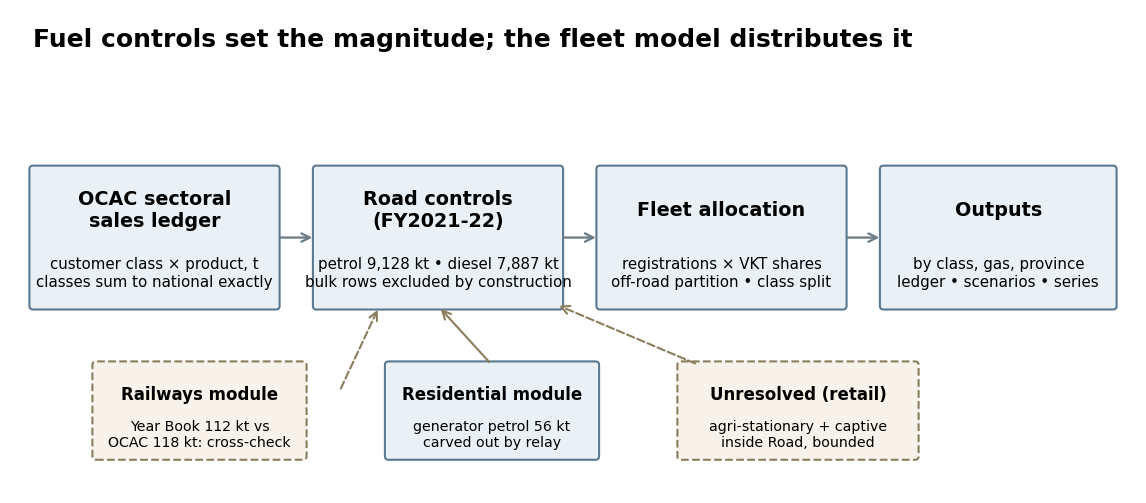
\includegraphics[width=0.92\linewidth]{transport_framework.png}
\caption{The calculation, end to end: the OCAC customer-class ledger supplies the road
controls, the fleet model distributes them, and the cross-sector relays (railways as a
cross-check, residential as a carve-out) and the unresolved retail claimants are explicit
boxes rather than prose. The high petrol share of the controls is consistent with
Pakistan's large two-wheeler fleet.}
\label{fig:activity}
\end{figure*}

\subsection{A provenance audit: the superseded control}

The previous edition anchored on national supply figures derived from the Economic
Survey's provisional nine-month FY2025 data. Those stored values---\SI{10162}{} and
\SI{8820}{\kilo\tonne}---were arithmetically inconsistent with their own source note: they
equal the nine-month figures times $16/9$, not the documented $12/9$ annualisation, an
annualisation applied twice. The diesel figure coincidentally landed within one percent of
the FY2021--22 \emph{national} internal HSD total, so the matched-year EDGAR comparison
looked right on a wrong-provenance number; the petrol figure overshot the fiscal-year
national total by eleven percent. A match against a benchmark is not provenance. The
superseded pair is retained as a named, executable boundary scenario
(\texttt{legacy\_pes\_control}, Section~\ref{sec:results}) rather than deleted---the same
discipline the residential sector applies to its superseded dung basis---so the bridge
from previously published numbers stays open and honest.

\subsection{What the road rows still include that they should not}

A customer class cannot see end uses. Retail pumps sell diesel to trucks, but also to
tube-well and thresher owners (stationary agriculture, IPCC 1A4c~i) and to captive
generator operators (1A2); retail petrol includes fuel carried home for household
generators (1A4b). One of these three is carved out---the generator petrol, relayed from
the residential module (Section~\ref{sec:methods})---and the two diesel claimants remain
inside, unresolved, biasing the road residual high conditional on the other deductions.
Two observations frame them: OCAC books \emph{zero} bulk HSD to its Agriculture row in
all ten editions, so the agricultural claim is retail-channel only; and the road share
of national diesel spans 0.83--0.91 across the ten-year panel---a customer-class
boundary sensitivity that bounds the sales channel, not the contamination within it,
which is priced separately by the retail non-road scenarios of
Section~\ref{sec:results}. The complete claimant
structure---observed bulk rows, carve-outs, residuals and unresolved status rows---is
the two-tier fuel ledger of Table~\ref{tab:ledger}.

\subsection{The fleet model}

Vehicle classes and their shares come from the national registration statistics
\citep{provregstats}, which give counts by class and province. Annual vehicle-kilometres
and fuel-split shares by class come from the transport parameter table, whose survival
parameters derive from a district-level Punjab transport manuscript \citep{naveedpunjab}
that adopts the survival functions of \citet{guttikunda2024}.

The classes are two- and three-wheelers, four-wheelers in three size bands, light and heavy
duty vehicles, buses, and an off-road class. That last one is a genuine complication rather
than a clean category, and Section~\ref{sec:limitations} treats it: the source workbook maps
its catch-all "other vehicles" entry into off-road wholesale, so the class is a residual as
well as a machinery category, and it is reported under the mixture-declaring name
\emph{Mixed off-road (1A4c/1A2)}.

\subsection{Air-pollutant factors}

The exploratory air-pollutant diagnostic (\ref{sec:air}) applies per-kilometre
factors to the same survival-weighted vehicle-kilometres that distribute the fuel control
total. The factors are transcriptions from the Punjab emissions workbook, and carry no
primary citation---the source file has no provenance column, and no published provenance
for them has been located here. They are consistent in magnitude with European
exhaust-factor compilations, but that is a plausibility observation, not a citation, and
it is why the layer is reported as an appendix diagnostic with no policy weight
(Section~\ref{sec:limitations}). NMVOC is non-methane VOC and \NOx{} is reported as
NO$_2$-equivalent mass, the inventory-wide basis.

\subsection{What this inventory had not read}

Pakistan publishes no nationally representative vehicle-kilometre survey that this study
could identify, and no on-road fuel-economy measurement was found. Everything else this
sector once described as unobtained turned out to be a reading failure, twice.

Compressed natural gas was the first instance: a substantial CNG fleet whose fuel sits in
the gas statistics, absent from the sector entirely while the transport row of OGRA's
sector-wise gas consumption table---the same table this inventory already read for the
residential control total---sat unread \citep{ogra2024,ograarchive}. That row became the
sector's third fuel control, and the previous edition drew the lesson: not absent, unread.

The OCAC sectoral tables are the second instance, at larger stakes, and the lesson applied
to the sentence that drew it. Two editions of this paper described OCAC's product-by-sector
sales as published but not obtained here. They were in the repository throughout---forty-eight monthly editions carrying
CUMULATIVE national tables, fetched by the aviation sector for their jet-fuel columns,
indexed, hashed, and already read by the residential sector for a kerosene cell; a
distinct population from the thirty-six DIRECT single-month editions below, as the edition
inventory (\texttt{outputs/ocac\_edition\_inventory.csv}) now distinguishes. This edition anchors on them (Section~\ref{sec:methods}) and builds its provincial
allocation from area pages (Section~\ref{sec:results}). There is now a third episode of
the same lesson: an earlier edition borrowed FY2024--25's provincial shape on the claim
that the reference year's area pages were never published, while the thirty-six direct
monthly editions carrying them sat fetched and hash-pinned in the repository. All three
episodes are kept here, in the data section, as the clearest available statement of what
``not obtained'' usually means in practice.
